\documentclass[aspectratio=169,11pt,usenames,dvipsnames]{beamer}

% \usepackage[colorlinks=true,linkcolor=customblue, citecolor=hpred,urlcolor=customlightblue]{hyperref}

\usetheme{simple}

% packages
\usepackage{mathrsfs}  
\usepackage{cancel}
% \usepackage{caption}
% \usepackage{tikz}

\makeatother
\renewcommand{\thefootnote}{\color{customblue}\faPaperPlaneO}
\makeatletter

\newcommand{\symfootnote}[1]{%
\let\oldthefootnote=\thefootnote%
\stepcounter{mpfootnote}%
\addtocounter{footnote}{-1}%
\renewcommand{\thefootnote}{$\dagger$}%
\footnote{#1}%
\let\thefootnote=\oldthefootnote%
}

\newcommand\blfootnote[1]{%
  \begingroup
  \renewcommand\thefootnote{}\footnote{#1}%
  \addtocounter{footnote}{-1}%
  \endgroup
}

\usepackage{xcolor}
\usepackage{graphicx}
\usepackage{empheq}
\usepackage{physics}
\usepackage{svg}
\usepackage{bm}
\usepackage{amsmath}
\usepackage{amssymb}
\usepackage{annotate-equations}

\usepackage{appendixnumberbeamer}

\usepackage{relsize}

\usepackage{fontawesome}


\usetikzlibrary{decorations.pathreplacing, decorations.pathmorphing,calc,arrows,positioning}

% Custom colors

\definecolor{isred}{HTML}{81182d}
\definecolor{hpred}{HTML}{712A27}
\definecolor{hpblue}{HTML}{44545c}

\definecolor{customblue}{HTML}{3c9bb3}
\definecolor{customgreen}{HTML}{117877}
\definecolor{custompink}{HTML}{c35861}
\definecolor{customred}{HTML}{9d1700}
\definecolor{customyellow}{HTML}{e0ad04}
\definecolor{lightgray}{HTML}{a6a4a4}

\definecolor{lightcustomblue}{HTML}{aad1e6}
\definecolor{lightpink}{HTML}{ba8489}

\definecolor{starrymain}{HTML}{3B5B65}
\definecolor{starrysecond}{HTML}{719593}

\definecolor{ektgreen}{HTML}{047c73}
\definecolor{ektblue}{HTML}{065680}

\definecolor{angcorr}{HTML}{502d7e}

\definecolor{pinky}{HTML}{c35861}
\definecolor{ming}{HTML}{117877}

\definecolor{jyublue}{HTML}{002145}
\definecolor{jyured}{HTML}{e13126}
\definecolor{jyulightblue}{HTML}{909eae}

\definecolor{paldarkblue}{HTML}{0d1f2d}
\definecolor{pallightblue}{HTML}{2f586e}
\definecolor{paldarkgold}{HTML}{d2973b}
\definecolor{pallightgold}{HTML}{e8ca84}
\definecolor{palred}{HTML}{8c0e0f}

\definecolor{palblue}{HTML}{0d3672}
\definecolor{palteal}{HTML}{406f6b}
\definecolor{palgold}{HTML}{b99146}
\definecolor{palviolet}{HTML}{9F87AF}

\definecolor{raapink}{HTML}{ce93b5}
\definecolor{raablue}{HTML}{5c93b8}

\usepackage{etoolbox}
\setbeamertemplate{blocks}[rounded][shadow=false]
\setbeamercolor{block title}{use=structure,fg=palteal,bg=palteal!10}
\setbeamercolor{block body}{parent=normal text,use=block title,bg=palteal!10}

\usepackage[most]{tcolorbox}
\newtcolorbox{mybox}[2][]{tcbox width=auto limited,capture=hbox,colbacktitle=red!10!white, colback=blue!10!white,coltitle=red!70!black, title={#2},fonttitle=\bfseries,#1}

\newtcolorbox{custombox}[3][]{%
    enhanced jigsaw,%
    colback=#3!5,%
    colframe=#3,%
    colbacktitle=#3!5,
    coltext=normal,
    center title,
    % size=small,%
    hbox,%
    center title,%
    % boxrule=1pt,%
    % title=\textbf{\textit{Example}},%
    % halign title=flush left,%
    coltitle=#3,%
    breakable,%
    boxrule=1.1pt,
    titlerule=0pt,
    left=-3pt,
    right=-3pt,
    top=2pt,
    bottom=0pt,
    enlarge left by=-0.1cm,
    grow to right by=0.21cm,
    title={#2},fonttitle=\bfseries\large,#1
}
\newtcolorbox{custombox2}[3][]{%
    enhanced jigsaw,%
    colback=#3!10,%
    colframe=#3,%
    colbacktitle=#3!10,
    coltext=normal,
    center title,
    % size=small,%
    hbox,%
    center title,%
    % boxrule=1pt,%
    % title=\textbf{\textit{Example}},%
    % halign title=flush left,%
    coltitle=#3,%
    breakable,%
    boxrule=0pt,
    titlerule=0pt,
    left=-8pt,
    right=-8pt,
    top=2pt,
    bottom=0pt,
    enlarge left by=-0.1cm,
    grow to right by=0.21cm,
    title={#2},fonttitle=\bfseries\large,#1
}
\newtcolorbox{custombox2transp}[3][]{%
    enhanced jigsaw,%
    colback=#3!4,%
    colframe=#3,%
    colbacktitle=#3!4,
    coltext=normal,
    center title,
    % size=small,%
    hbox,%
    center title,%
    % boxrule=1pt,%
    % title=\textbf{\textit{Example}},%
    % halign title=flush left,%
    coltitle=#3,%
    breakable,%
    boxrule=0pt,
    titlerule=0pt,
    left=-8pt,
    right=-8pt,
    top=2pt,
    bottom=0pt,
    enlarge left by=-0.1cm,
    grow to right by=0.21cm,
    title={#2},fonttitle=\bfseries\large,#1
}
\newtcolorbox{untitledcustombox}{%
    enhanced jigsaw,%
    colback=palteal!10,%
    colframe=palteal,%
    % colbacktitle=#1!10,
    coltext=normal,
    % center title,
    % size=small,%
    hbox,%
    center title,%
    % boxrule=1pt,%
    % title=\textbf{\textit{Example}},%
    % halign title=flush left,%
    % coltitle=#1,%
    breakable,%
    boxrule=0pt,
    titlerule=0pt,
    left=-2pt,
    right=-2pt,
    top=2pt,
    bottom=1pt,
    enlarge left by=-0.1cm,
    grow to right by=0.21cm,
}
\newtcolorbox{untitledcustomboxtransp}{%
    enhanced jigsaw,%
    colback=palteal!4,%
    colframe=palteal,%
    % colbacktitle=#1!10,
    coltext=normal,
    % center title,
    % size=small,%
    hbox,%
    center title,%
    % boxrule=1pt,%
    % title=\textbf{\textit{Example}},%
    % halign title=flush left,%
    % coltitle=#1,%
    breakable,%
    boxrule=0pt,
    titlerule=0pt,
    left=-2pt,
    right=-2pt,
    top=2pt,
    bottom=1pt,
    enlarge left by=-0.1cm,
    grow to right by=0.21cm,
}
\usepackage{varwidth}

\hypersetup{colorlinks,linkcolor=normal,citecolor=customblue, citecolor=pinky,urlcolor=pinky}

% custom commands
\newcommand{\coloredeq}[2]{\begin{empheq}[box=\colorbox{#1}]{align*}#2\end{empheq}}
\newcommand\scalemath[2]{\scalebox{#1}{\mbox{\ensuremath{\displaystyle #2}}}}
\newcommand\coloreditem[1]{\item[\textcolor{#1}{\usebeamertemplate{itemize \beameritemnestingprefix item}}]}
\newcommand{\imp}[1]{{\sffamily\bfseries\color{customblue}#1}}

\setbeamertemplate{frametitle}[default][center]

\usepackage{etoolbox}% http://ctan.org/pkg/etoolbox
\makeatletter
\newlength{\secnamelength}
\newsavebox{\longestsec}% Box to save longest sectional heading
\patchcmd{\beamer@section}% <cmd>
  {\beamer@savemode}% <search>
  {\begin{lrbox}{\longestsec}#1\end{lrbox}%
   \ifdim\wd\longestsec>\secnamelength\relax\setlength{\secnamelength}{\wd\longestsec}\fi%
   \beamer@savemode}% <replace>
  {}{}% <success><failure>
\AtEndDocument{% http://tex.stackexchange.com/q/137495/5764
  \immediate\write\@auxout{\global\secnamelength=\the\secnamelength}%
}
\makeatother


\renewcommand{\d}{\mathrm{d}}
\renewcommand{\tr}[1]{\mathrm{Tr}\left\{#1\right\}}

\usepackage{scalerel}
\newcommand\Blacktriangleright{\raisebox{0.2em}{\scaleobj{0.7}{\blacktriangleright}}}

% customize beamer
% \setbeamercolor{frametitle}{fg=jyublue}
\setbeamercolor{framesubtitle}{fg=normal}
\setbeamercolor{subtitle}{fg=customblue}
% \setbeamerfont{frametitle}{series=\normalfont\huge}
\setbeamerfont{frametitle}{series=\normalfont\huge}
\setbeamerfont{framesubtitle}{series=\normalfont\normalsize}
\setbeamerfont{section in toc}{series=\normalfont\Large}
% \setbeamercolor{section in toc}{fg=red}
\setbeamerfont{subsection in toc}{series=\normalfont\small}
% \setbeamerfont{subsection in toc}{series=\itshape}

% all subsections in TOC in a single line
\defbeamertemplate*{subsection in toc}{sub on 1 line}
{
  \ifnum\inserttocsubsectionnumber=1
    \vspace{0.1cm}\hspace{0.45cm}\inserttocsubsection
  \else
    {\color{normal}$\sbullet[0.6]$}\hspace{0.2cm}\inserttocsubsection
  \fi
}


\usefonttheme[onlymath]{serif}

% Item shape and color
\setbeamertemplate{itemize item}{\raisebox{0.2em}{\scalebox{0.7}{${\color{customblue}\blacktriangleright}$}}} 

\newcommand{\itemcolor}[1]{\setbeamertemplate{itemize item}{\raisebox{0.2em}{\scalebox{0.7}{${\color{#1}\blacktriangleright}$}}}}
\addtobeamertemplate{navigation symbols}{}{%
    \usebeamerfont{footline}%
    \usebeamercolor[fg]{footline}%
    \hspace{1em}%
    \insertframenumber/\inserttotalframenumber
}
\setbeamercolor{footline}{fg=customblue}
\setbeamerfont{footline}{series=\normalfont\footnotesize}
\setbeamertemplate{navigation symbols}{}

% scale bullet symbol
\newcommand\sbullet[1][.5]{\mathbin{\vcenter{\hbox{\scalebox{#1}{$\bullet$}}}}}

% colored box environment
\usepackage{tcolorbox}
\tcbuselibrary{skins,hooks}
\newcommand\fancybox[3]{%
\tcbset{
    mybox/.style={
        enhanced,
        boxsep=0mm,
        opacityfill=0,
        overlay={
            \coordinate (X) at ([xshift=2mm, yshift=-1.5mm]frame.north east);
            \node[align=left, text=#1, text width=5cm, anchor=north west] at (X) {#2};
            \draw[line width=0.3mm, color=#1] (frame.north east) -- (frame.south east); 
            }
        }
    }

\begin{tcolorbox}[mybox]
    #3
\end{tcolorbox}
}

% figure caption
\usepackage{caption}
\captionsetup[figure]{labelformat=empty}

% title page
\title{\normalfont\bfseries\Large Transport of {\color{jyublue}jets} and {\color{jyublue}heavy quarks} in the\\
 {\color{jyured}glasma} pre-equilibrium stage\vspace{-10pt}}
\date{\vspace{-20pt}
    \begin{center}
        \resizebox{.9\textwidth}{!}{%
        
\includegraphics[height=0.7cm]{images/university-of-jyvaskyla-logo-freelogovectors.net_.png}%
        \quad
        
\includegraphics[height=0.7cm]{images/HIP_Logo_EN_V4_Pos_Blue.pdf}%
        \quad
        
\includegraphics[height=0.75cm]{images/CoE-logo-01_nobg.png}%
        \quad
        
\includegraphics[height=0.8cm]{images/AKA_EN_pysty_sininen_RGB.png}%
        \quad
        
\includegraphics[height=0.7cm]{images/Logo-ERC-black_0.png}%
        }
    \end{center}

    \begin{columns}
        \begin{column}{0.1\textwidth}\end{column}
        \begin{column}{0.8\textwidth}
            \centering
            \footnotesize High energy probes of the initial stages, CERN, March 2025\end{column}
        \begin{column}{0.1\textwidth}\end{column}
    \end{columns}    
}
\author{\vspace{-20pt}{\large {\color{jyured} $\displaystyle\int\mathcal{DA}$}vramescu}\\[22pt]{\scriptsize\itshape U. Jyväskylä, HIP}\\[10pt]}
\institute{\vspace{-22pt}
\begin{center}
    Showcasing results done in collaboration with
\end{center}
\begin{columns}
    \begin{column}{0.22\textwidth}
      \centering
      \footnotesize{\color{jyublue}T. Lappi, H. M\"{a}ntysaari}\\
      {\scriptsize\itshape U. Jyväskylä, HIP}
    \end{column}
    \begin{column}{0.16\textwidth}
      \centering
      \footnotesize{\color{jyublue}A. Ipp, D. M\"{u}ller}\\
      {\scriptsize\itshape TU Wien}
    \end{column}
    \begin{column}{0.2\textwidth}
      \centering
      \footnotesize{\color{jyublue}V. Greco, M. Ruggieri}\\
      {\scriptsize\itshape U. Catania, INFN-LNS}
    \end{column}
    \begin{column}{0.3\textwidth}
        \centering
        \footnotesize{\color{jyublue}C. Lamas, M. Li, C. A. Salgado}\\
        {\scriptsize\itshape IGFAE, U. Santiago de Compostela}
      \end{column}
\end{columns}
\vspace{10pt}
}

\usebackgroundtemplate{
\tikz[overlay,remember picture] \node[opacity=0.1, at=(current page.center)] {
   
\includegraphics[height=0.7\paperheight]{images/CoE-QM-2_2-modified.png}};
}

\setbeamercolor{progress bar progress}{use=progress bar,bg=progress bar.fg}
\defbeamertemplate{footline}{progress bar}{
  \dimen0=\paperwidth
  \multiply\dimen0 by \insertframenumber
  \divide\dimen0 by \inserttotalframenumber
  \edef\progressbarwidth{\the\dimen0}

  \leavevmode%
  \begin{beamercolorbox}[wd=\paperwidth,ht=0.08cm]{progress bar}
    \begin{beamercolorbox}[wd=\progressbarwidth,ht=0.1cm]{progress bar progress}
    \end{beamercolorbox}%
  \end{beamercolorbox}%
}


\usepackage{tikz}

\definecolor{color1}{RGB}{173,216,230}
\definecolor{color2}{RGB}{255,140,0}

\newcounter{totavalue}
\newcounter{parvalue}

\def\aux{4}
\def\radius{12pt}
\def\innerradius{7pt}
\def\step{6pt}

\newcommand\circcounter{%
\ifnum\inserttotalframenumber<2\relax
\else
  \setcounter{totavalue}{\inserttotalframenumber}
  \setcounter{parvalue}{\insertframenumber}
  \ifnum\inserttotalframenumber>45\relax
    \renewcommand\step{0pt}
  \fi%
  \pgfmathsetmacro{\aux}{360/\thetotavalue}
  \begin{tikzpicture}[remember picture,overlay,rotate=90+\aux]
  \foreach \i in {0,1,...,\thetotavalue}
    \fill[palteal!40] 
      (0,0) -- (-\i*\aux:\radius) arc  (-\i*\aux:-(\i+1)*\aux+\step:\radius) -- cycle;
  \foreach \i in {1,...,\insertframenumber}
    \fill[palteal] 
      (0,0) -- (-\i*\aux:\radius) arc  (-\i*\aux:-(\i+1)*\aux+\step:\radius) -- cycle;
  \fill[white] circle (\innerradius);
  \node at (0,0) {\footnotesize\insertframenumber}; 
  % \node at (0,0) {}; 
  \end{tikzpicture}%
\fi%
}

\begin{document}

%%%%%%%%%%%%%%%%%%%%%%%%%%%%%%%%%%%%%%%%%%%%%%%%%%%%%%%%%
%%%%%%%%%%%%%%%%%%%%%% TITLE SLIDE %%%%%%%%%%%%%%%%%%%%%%
%%%%%%%%%%%%%%%%%%%%%%%%%%%%%%%%%%%%%%%%%%%%%%%%%%%%%%%%%

\maketitle
\usebackgroundtemplate{ } 

%%%%%%%%%%%%%%%%%%%%%%%%%%%%%%%%%%%%%%%
%%%%%%%%%%%%%%%%% TOC %%%%%%%%%%%%%%%%%
%%%%%%%%%%%%%%%%%%%%%%%%%%%%%%%%%%%%%%%


\setbeamertemplate{background}{
\tikz[overlay,remember picture] \node[opacity=0.15, at=(current page.center), align=center] {
    \\[15pt]
    {\transparent{0.2}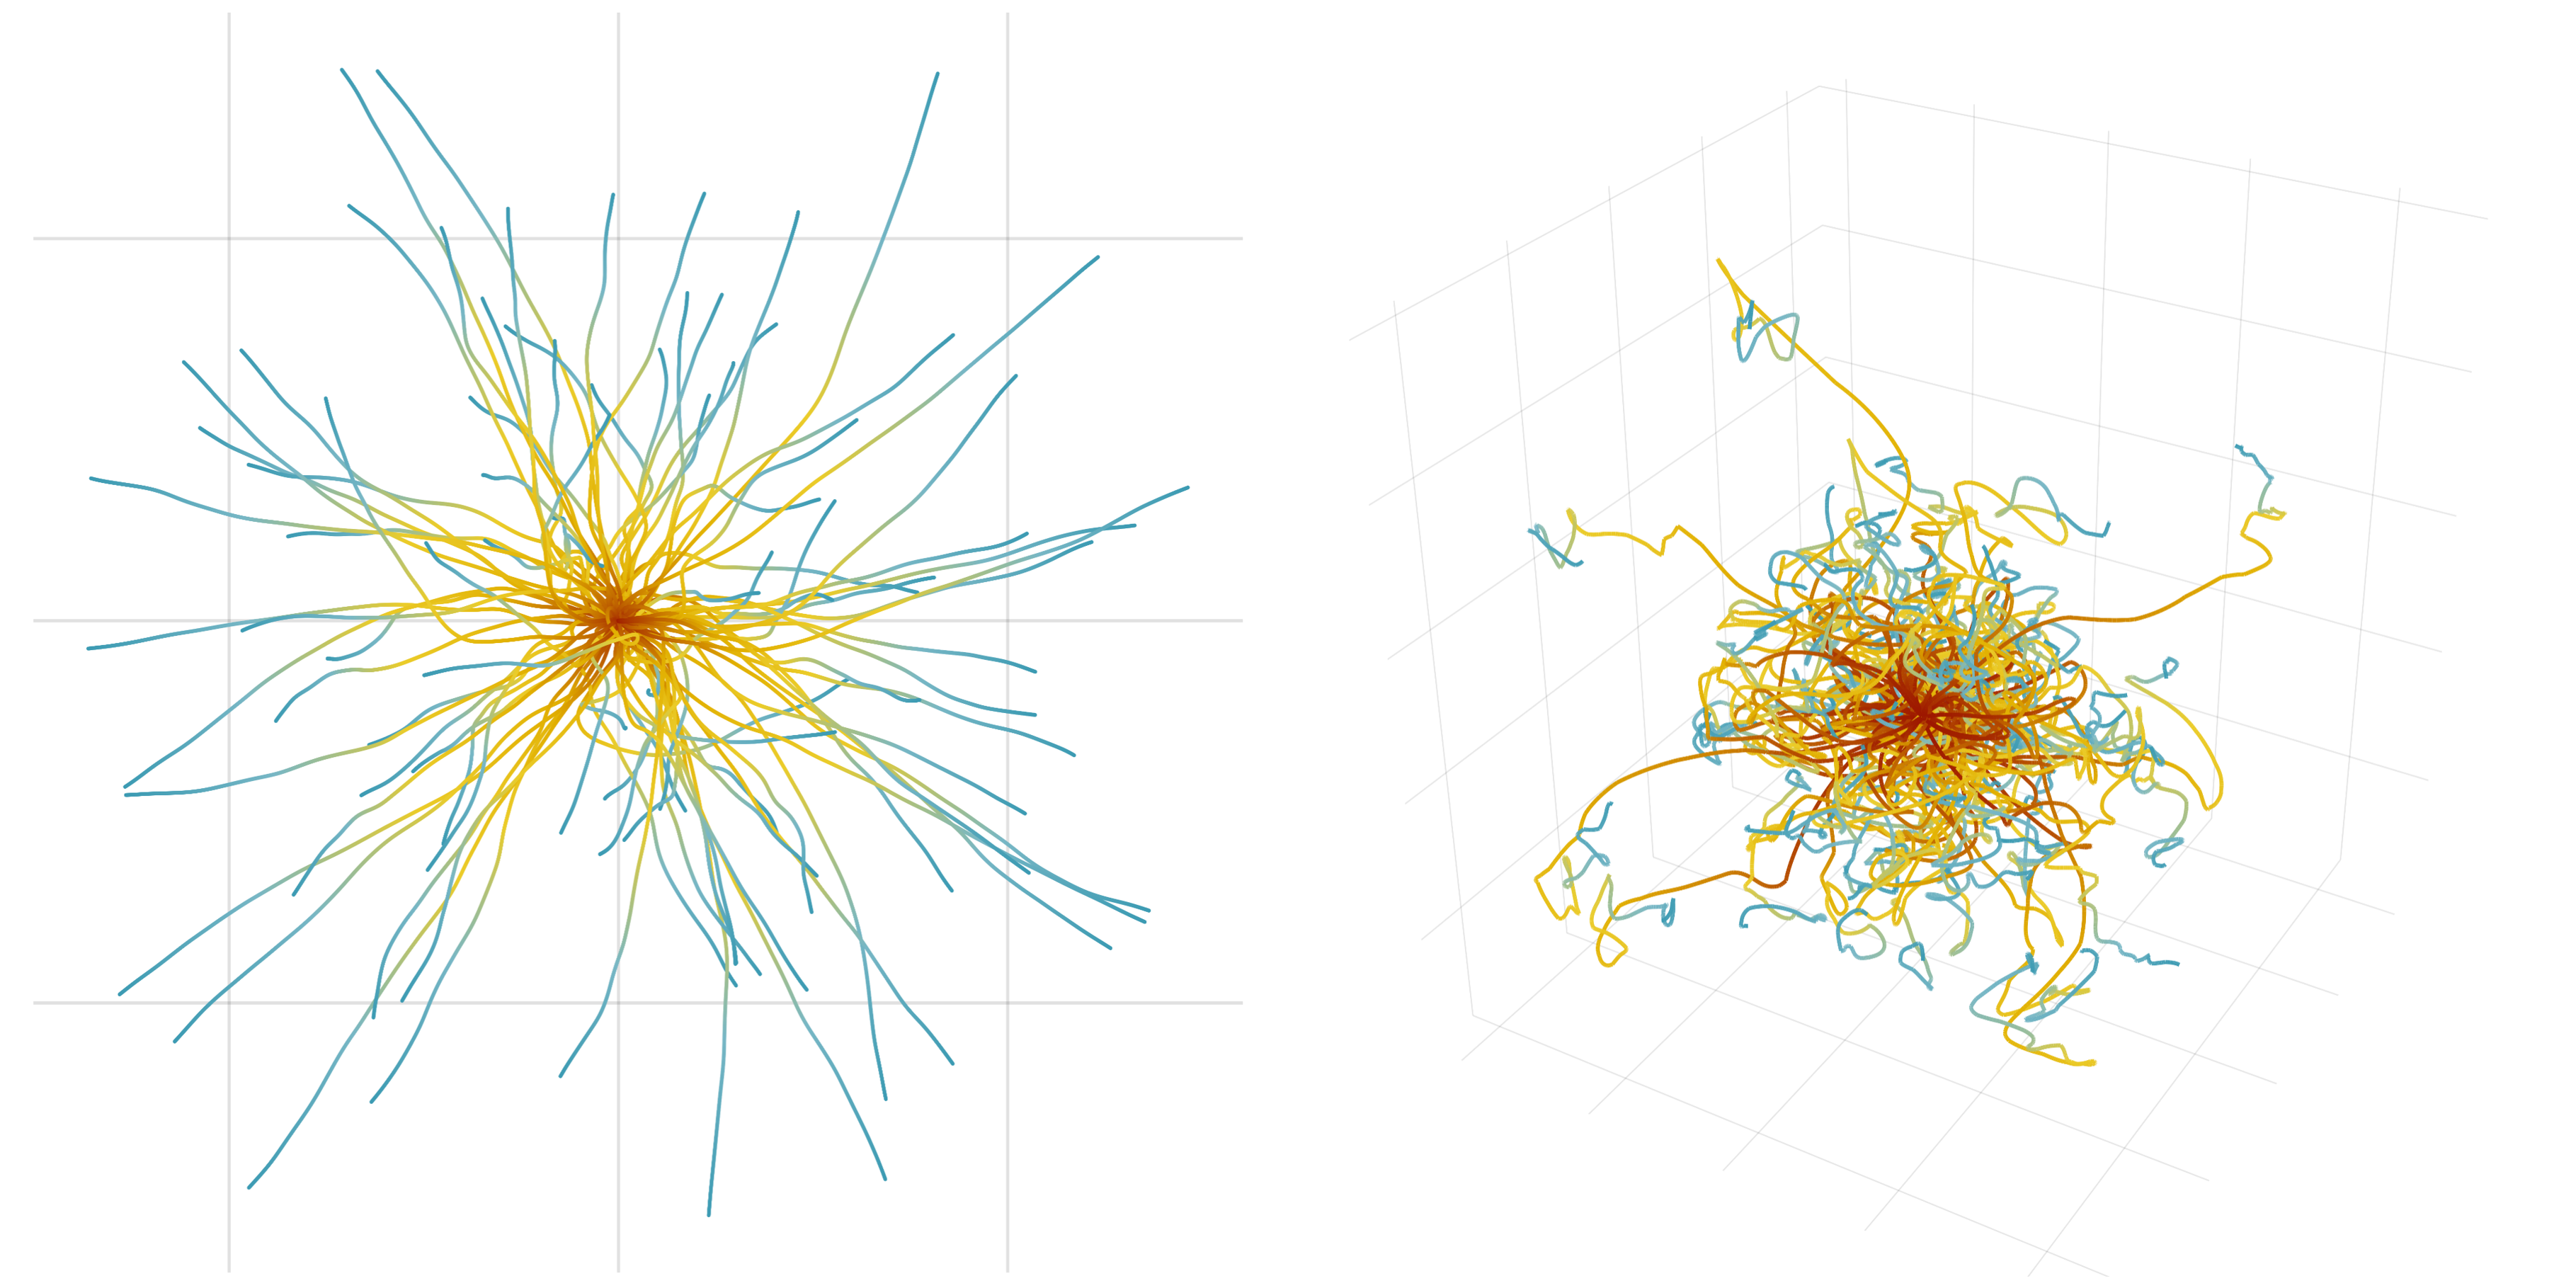
\includegraphics[height=0.7\paperheight]{images/trajectories_cpic.png}} 
    \\[10pt]  
   };
}
\begin{frame}{Outline}
    \begin{center}
        \tableofcontents
    \end{center}
\end{frame}
\setbeamertemplate{background}{}

\setcounter{framenumber}{0}
\setbeamertemplate{footline}[progress bar]
\setbeamercolor{progress bar}{fg=palteal,bg=palteal!40}
\addtobeamertemplate{headline}{}{\vspace{1cm}\hfill\circcounter\hspace*{1cm}}
\addtobeamertemplate{frametitle}{\vspace{-0.8cm}}{}

%%%%%%%%%%%%%%%%%%%%%%%%%%%%%%%%%%%%%%%%%
%%%%%%%%%%%%%%%% SECTION %%%%%%%%%%%%%%%%
%%%%%%%%%%%%%%%%%%%%%%%%%%%%%%%%%%%%%%%%%

\section{Introduction}

%%%%%%%%%%%%%%%%%%%%%%%%%%%%%%%%%%%%%%%%%
%%%%%%%%%%%%%% SUBSECTION %%%%%%%%%%%%%%%
%%%%%%%%%%%%%%%%%%%%%%%%%%%%%%%%%%%%%%%%%

\subsection{Stages}

%%%%%%%%%%%%%%%%%%%%%%%%%%%%%%%%%%%%%%%%%
%%%%%%%%%%%%%%%%% SLIDE %%%%%%%%%%%%%%%%%
%%%%%%%%%%%%%%%%%%%%%%%%%%%%%%%%%%%%%%%%%

\begin{frame}
    \frametitle{Heavy-ion collisions}
    \framesubtitle{Stages at weak coupling}
    \vspace{-15pt}
    \begin{columns}[onlytextwidth,t]
        \column{.02\textwidth}
        \column{.47\textwidth}
            \begin{center}
                \vspace{-5pt}
                \begin{tikzpicture}
                    \node[anchor=south west,inner sep=0] at (0,0) {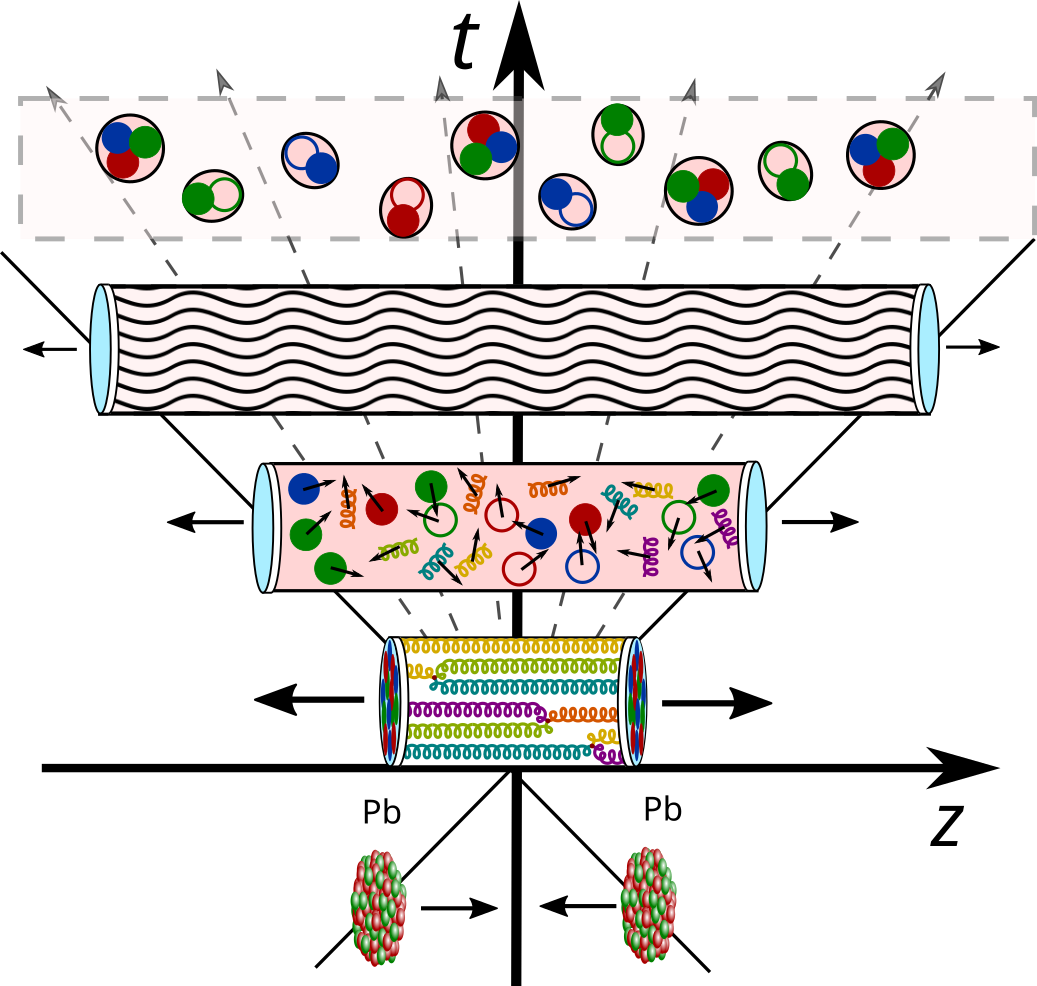
\includegraphics[width=0.95\textwidth]{images/cover_figure_A01.png}};
                \end{tikzpicture}
            \end{center}
        \column{.02\textwidth}
        \column{.47\textwidth}
            \vspace{10pt}
            \begin{center}
            \begin{custombox2}{\color{normal}Collision stages}{lightgray}
                \small
                \begin{varwidth}{0.8\textwidth}
                \begin{itemize}\itemsep0em 
                    \setbeamertemplate{itemize item}{\raisebox{0.2em}{\scalebox{0.7}{${\color{normal}\blacktriangleright}$}}} 
                    \item {Before collision {\scriptsize $\tau\leq 0\,\mathrm{fm/c}$}}\\[1pt]
                        {\color{lightgray}\scriptsize Gluon field of high-energy nucleus}
                    \setbeamertemplate{itemize item}{\raisebox{0.2em}{\scalebox{0.7}{${\color{palviolet}\blacktriangleright}$}}} \item {{\bfseries\color{palviolet} Initial stage} {\scriptsize $\tau\lesssim
                    0.3\,\mathrm{fm/c}$}}\\[1pt]
                        {\color{lightgray}\scriptsize {\bfseries\color{palviolet}Glasma} strong classical gluon fields}
                    \setbeamertemplate{itemize item}{\raisebox{0.2em}{\scalebox{0.7}{${\color{normal}\blacktriangleright}$}}} \item Thermalization {\scriptsize$\tau\lesssim
                    1\,\mathrm{fm/c}$}\\[1pt] 
                        {\color{lightgray}\scriptsize Effective kinetic theory} 
                        % \\ {\color{lightgray}\scriptsize Quasiparticle distribution function}
                    \item Equilibration {\scriptsize $\tau\lesssim 10\,\mathrm{fm/c}$}\\[1pt]
                    {\color{lightgray}\scriptsize Relativistic hydrodynamics} 
                    % \\ {\color{lightgray}\scriptsize Energy-momentum tensor}
                    \item Final stages {\scriptsize $\tau\geq 10\,\mathrm{fm/c}$}\\[1pt]
                    {\color{lightgray}\scriptsize Particlization, hadronization}
                \end{itemize}
                \end{varwidth}
            \end{custombox2}
            \end{center}
        \column{.02\textwidth}
    \end{columns}
    \blfootnote{\scriptsize Berges, Heller, Mazeliauskas, Venugopalan \href{https://arxiv.org/abs/2005.12299}{{\color{palgold}\texttt{[2005.12299]$^\text{\tiny\faExternalLink}$}}}, Schlichting, Teaney \href{https://arxiv.org/abs/1908.02113}{{\color{palgold}\texttt{[1908.02113]$^\text{\tiny\faExternalLink}$}}}}
\end{frame}

\subsection{Initial stage}

%%%%%%%%%%%%%%%%%%%%%%%%%%%%%%%%%%%%%%%%%
%%%%%%%%%%%%%%%%% SLIDE %%%%%%%%%%%%%%%%%
%%%%%%%%%%%%%%%%%%%%%%%%%%%%%%%%%%%%%%%%%

\begin{frame}[noframenumbering]
    \frametitle{Initial stage of collision}
    % \framesubtitle{Stages at weak coupling}
    \vspace{-10pt}
    \begin{columns}[onlytextwidth,t]
        \column{.02\textwidth}
        \column{.47\textwidth}
            \begin{center}
                \vspace{-5pt}
                \begin{tikzpicture}
                    \node[anchor=south west,inner sep=0] at (0,0) {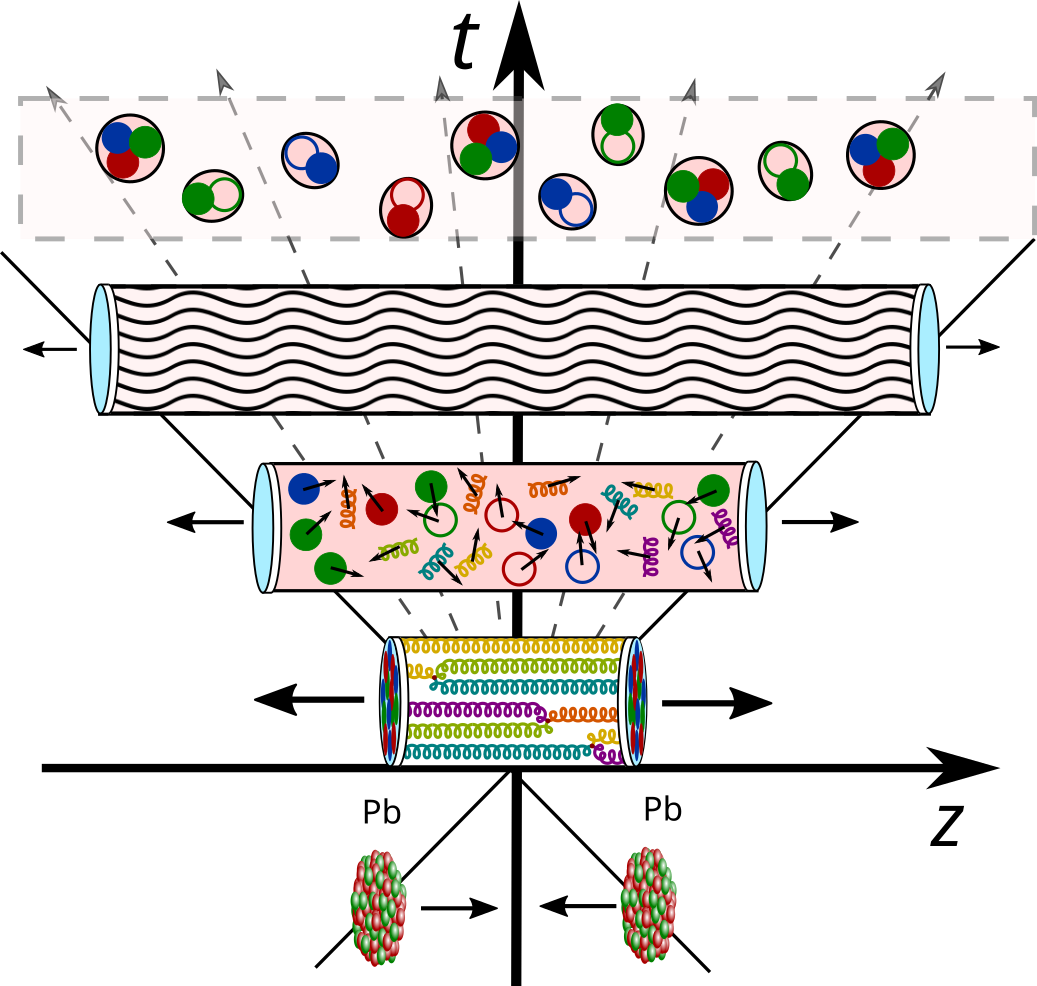
\includegraphics[width=0.95\textwidth]{images/cover_figure_A01.png}};
                    \draw<1>[white, fill=white, fill opacity=0.9] (0.0,2.45) rectangle (6.8,6.5);
                    \draw<1>[palviolet,thick,fill=palviolet,fill opacity=0.1,rounded corners=3pt] (0.1,-0.1) rectangle (6.7,2.45);
                \end{tikzpicture}
            \end{center}
        \column{.02\textwidth}
        \column{.47\textwidth}
            \vspace{7pt}
            \begin{center}
            \begin{custombox2}{Glasma initial stage}{palviolet}
                \small
                \begin{varwidth}{0.76\textwidth}
                \begin{itemize}\itemsep0em 
                    \setbeamertemplate{itemize item}{\raisebox{0.2em}{\scalebox{0.7}{${\color{palviolet}\blacktriangleright}$}}} 
                    \item {Color glass condensate}\\[1pt]
                        {\color{lightgray}\scriptsize QCD in the high-energy limit}
                    \item Weakly coupled $\alpha_s\ll 1$
                    \item {\bfseries Classical gluon fields}\\[1pt]
                        {\color{lightgray}\scriptsize Occupation number $\sim 1/\alpha_s\gg 1$}
                    \item {\bfseries Non-perturbative} regime
                    % \item {\bfseries Lattice gauge theory}\\[1pt]
                        % {\color{lightgray}\scriptsize Numerical solution}
                    \item {\bfseries Out-of-equilibrium} medium
                    
                \end{itemize}
                \end{varwidth}
            \end{custombox2}

            \begin{custombox2}{Hard probes}{palteal}
                \small
                \begin{varwidth}{0.68\textwidth}
                \begin{itemize}\itemsep0em 
                    \setbeamertemplate{itemize item}{\raisebox{0.2em}{\scalebox{0.7}{${\color{palteal}\blacktriangleright}$}}} 
                    \item Heavy quarks and jets\\[1pt]
                    {\color{lightgray}\scriptsize Produced in the initial stage}
                \end{itemize}
                \end{varwidth}
            \end{custombox2}
            \end{center}
        \column{.02\textwidth}
    \end{columns}
    \blfootnote{\scriptsize Lappi \href{https://arxiv.org/abs/hep-ph/0606207}{{\color{palviolet}\texttt{[hep-ph/0606207]}$^\text{\tiny\faExternalLink}$}}, Gelis \href{https://arxiv.org/abs/1211.3327}{{\color{palviolet}\texttt{[1211.3327]}$^\text{\tiny\faExternalLink}$}}}
\end{frame}


%%%%%%%%%%%%%%%%%%%%%%%%%%%%%%%%%%%%%%%%%
%%%%%%%%%%%%%% SUBSECTION %%%%%%%%%%%%%%%
%%%%%%%%%%%%%%%%%%%%%%%%%%%%%%%%%%%%%%%%%

\subsection{Hard probes}

%%%%%%%%%%%%%%%%%%%%%%%%%%%%%%%%%%%%%%%%%
%%%%%%%%%%%%%%%%% SLIDE %%%%%%%%%%%%%%%%%
%%%%%%%%%%%%%%%%%%%%%%%%%%%%%%%%%%%%%%%%%

\setbeamertemplate{background}{
\tikz[overlay,remember picture] \node[at=(current page.center), align=center] {\\[10pt]
{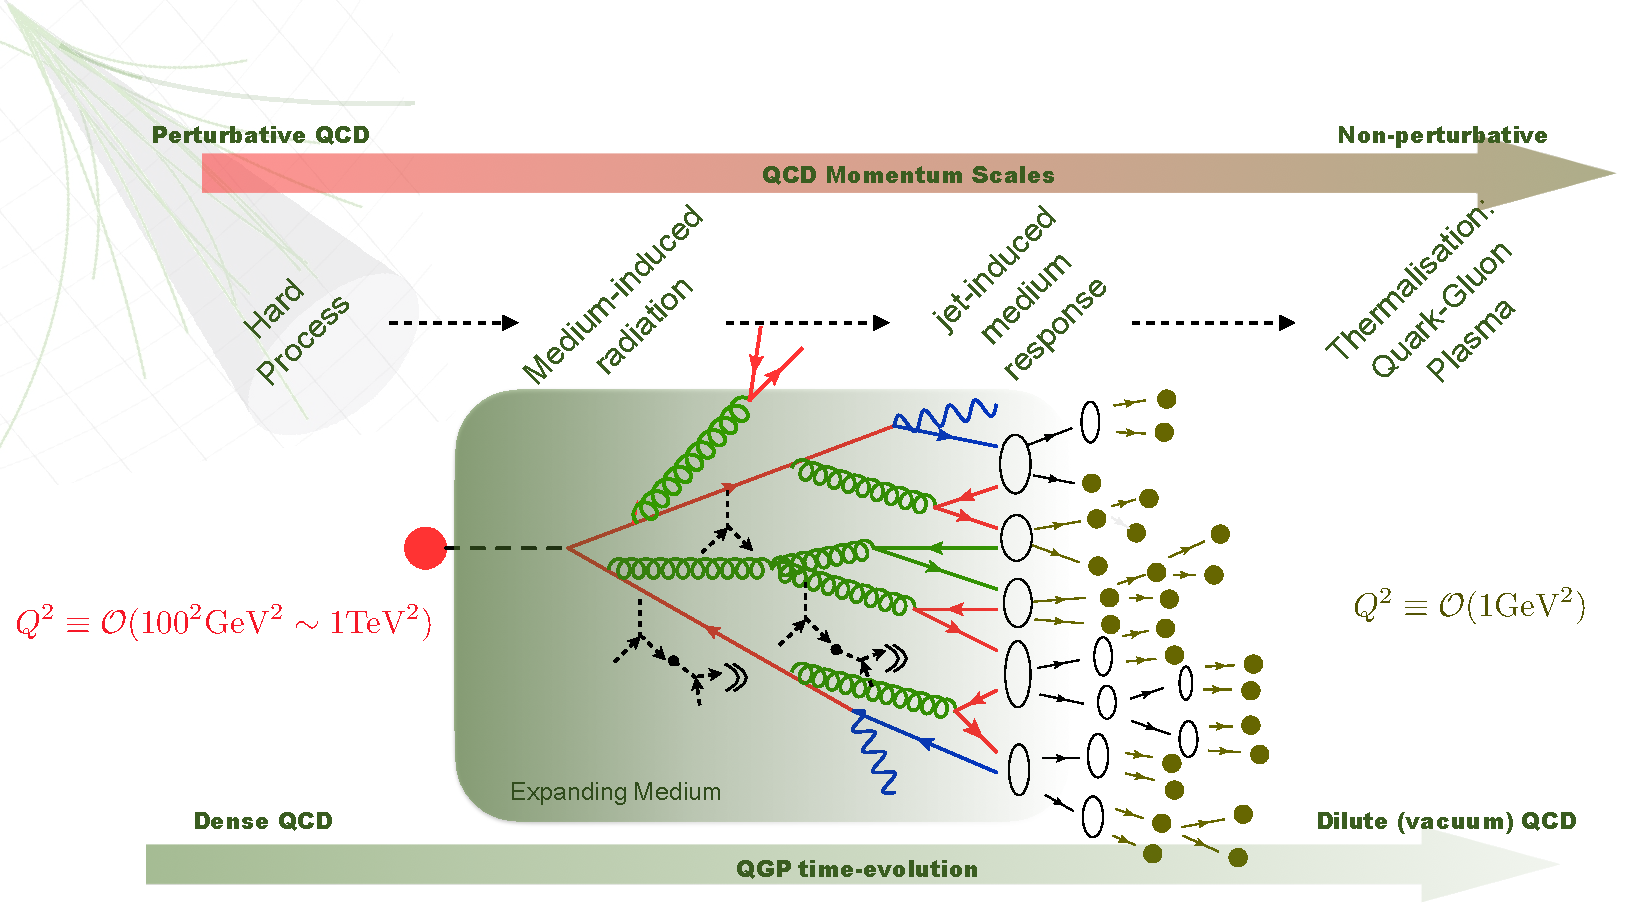
\includegraphics[height=0.8\paperheight]{images/Holmganga_jets_Liliana-scales.pdf}}};
}
\begin{frame}
    \frametitle{Jets as probes}
    \framesubtitle{Stages and scales of interest}
    \blfootnote{\scriptsize Apolinario - \textit{Jetography via the Quark-Gluon Plasma} \href{https://indico.cern.ch/event/1385550/}{{\color{red}\texttt{[CERN 24]$^\text{\tiny\faExternalLink}$}}}}
\end{frame}
\setbeamertemplate{background}{}

%%%%%%%%%%%%%%%%%%%%%%%%%%%%%%%%%%%%%%%%%
%%%%%%%%%%%%%%%%% SLIDE %%%%%%%%%%%%%%%%%
%%%%%%%%%%%%%%%%%%%%%%%%%%%%%%%%%%%%%%%%%

\setbeamertemplate{background}{
\tikz[overlay,remember picture] \node[at=(current page.center), align=center] {\\[-5pt]
{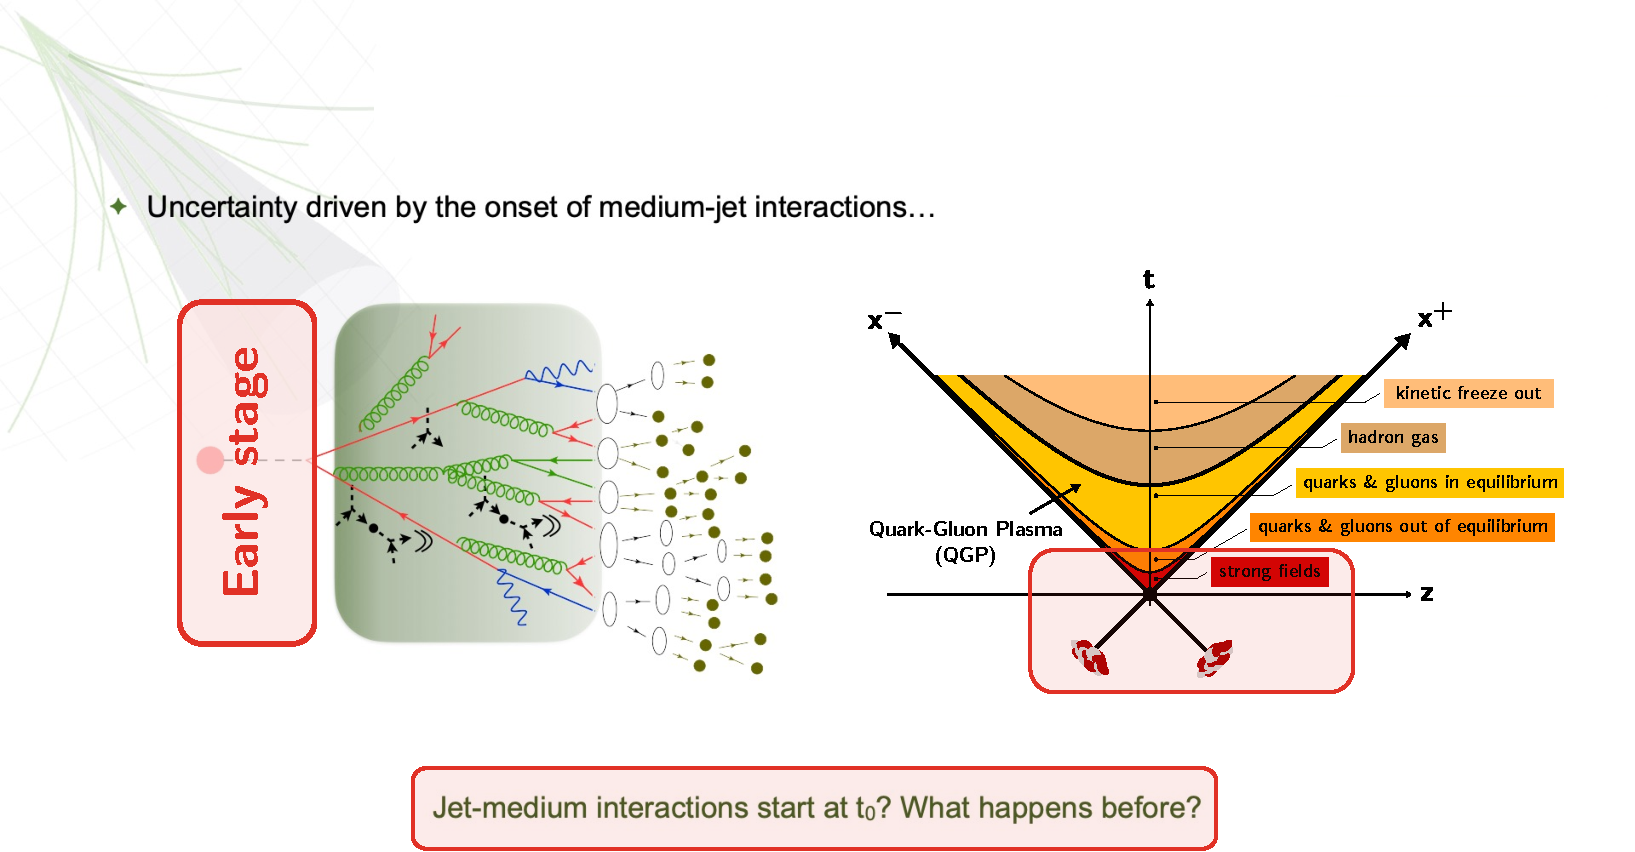
\includegraphics[height=0.8\paperheight]{images/LApolinario_HP23-modelling-early.pdf}}};
}
\begin{frame}[noframenumbering]
    \frametitle{Jets as probes of the {\color{red}early stage}}
    % \framesubtitle{Stages and scales of interest}
    \blfootnote{\scriptsize Apolinario - \textit{Monte Carlo modeling of jets} \href{https://indico.uni-muenster.de/event/1409/contributions/2412/}{{\color{red}\texttt{[Plenary Hard Probes 23]$^\text{\tiny\faExternalLink}$}}}, adapted}
\end{frame}
\setbeamertemplate{background}{}

%%%%%%%%%%%%%%%%%%%%%%%%%%%%%%%%%%%%%%%%%
%%%%%%%%%%%%%%%%% SLIDE %%%%%%%%%%%%%%%%%
%%%%%%%%%%%%%%%%%%%%%%%%%%%%%%%%%%%%%%%%%

\begin{frame}
    \frametitle{Heavy quarks as probes}
    \framesubtitle{Approaches and kinematic regimes}

    \begin{columns}[onlytextwidth,t]
        \column{.02\textwidth}
        \column{.57\textwidth}
            \vspace{-20pt}
            \begin{center}
                \begin{tikzpicture}
                    \node[anchor=south west,inner sep=0] at (0,0) {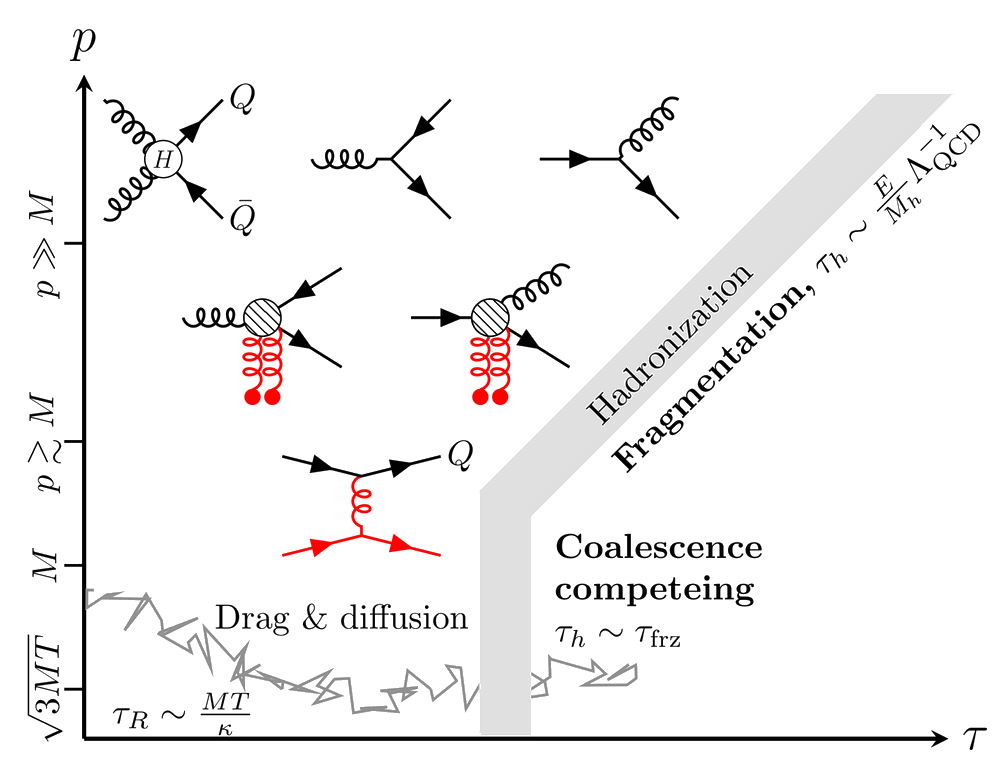
\includegraphics[width=0.95\textwidth]{images/HP24-Weiyao-Ke-HF-Theory-2-crop-white.png}};
                \end{tikzpicture}
            \end{center}
        \column{.02\textwidth}
        \column{.37\textwidth}
        \vspace{10pt}
        \begin{center}
            \begin{custombox2}{\color{normal}Approaches}{lightgray}
                \small
                \begin{varwidth}{0.85\textwidth}
                \begin{itemize}\itemsep0em 
                    \setbeamertemplate{itemize item}{\raisebox{0.2em}{\scalebox{0.7}{${\color{normal}\blacktriangleright}$}}} 
                    \item pQCD production\\[1pt]
                        {\color{lightgray}\scriptsize FONLL and GM-VFNS at NLO+NLL accuracy}
                    \item Transport models\\[1pt]
                        {\color{lightgray}\scriptsize Boltzmann, Langevin, Fokker-Planck equations}
                    \item Hadronization\\[1pt]
                        {\color{lightgray}\scriptsize Fragmentation + coalescence}  
                \end{itemize}
                \end{varwidth}
            \end{custombox2}
            \end{center}
        \column{.02\textwidth}
    \end{columns}

    \vspace{-5pt}    
    \blfootnote{\scriptsize Ke - \textit{Open Heavy Flavor: Theory} \href{https://indico.cern.ch/event/1339555/contributions/6038190/}{{\color{red}\texttt{[Plenary Hard Probes 24]$^\text{\tiny\faExternalLink}$}}}}
\end{frame}

%%%%%%%%%%%%%%%%%%%%%%%%%%%%%%%%%%%%%%%%%
%%%%%%%%%%%%%%%%% SLIDE %%%%%%%%%%%%%%%%%
%%%%%%%%%%%%%%%%%%%%%%%%%%%%%%%%%%%%%%%%%

\begin{frame}[noframenumbering]
    \frametitle{Heavy quarks as probes of the {\color{red}early stage}}
    % \framesubtitle{Recent focus on the early stage}

    \begin{center}
        \begin{tikzpicture}
            \node[anchor=south west,inner sep=0] at (0,0) {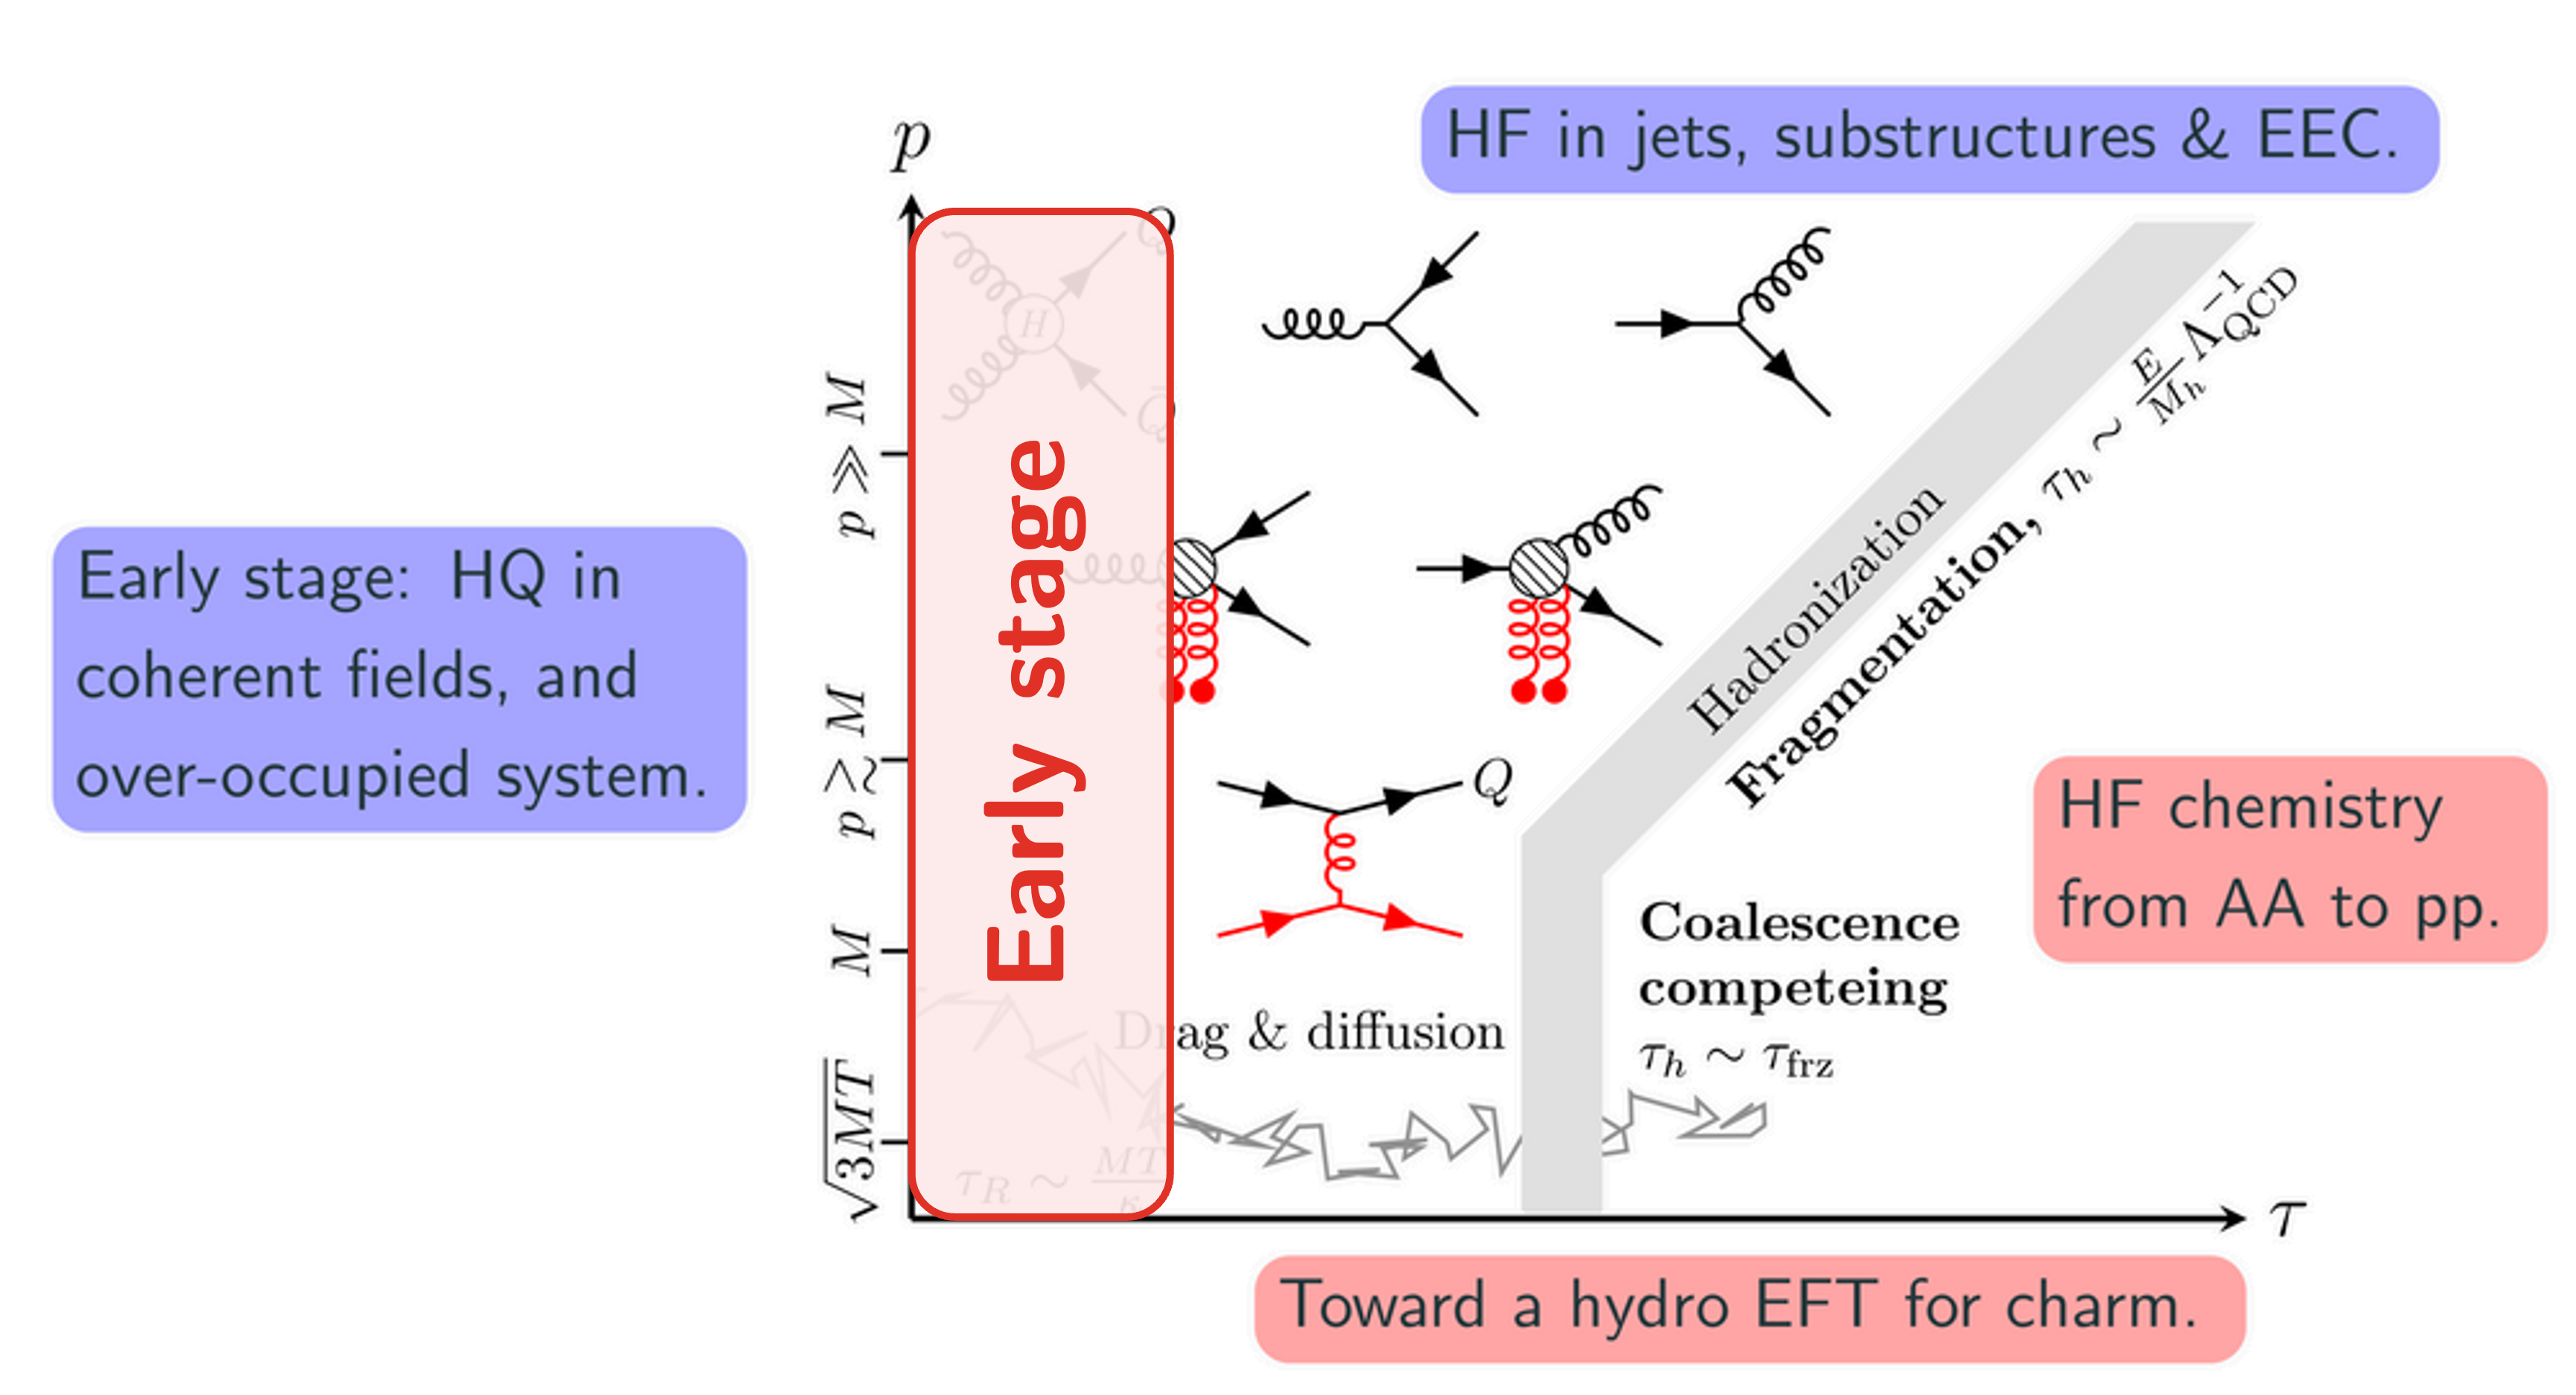
\includegraphics[width=0.8\textwidth]{images/HP24-Weiyao-Ke-HF-Theory-28-crop-white-edit.png}};
            % \draw<1>[palgold,thick,fill=palgold,fill opacity=0.1,rounded corners=3pt] (0.0,4) rectangle (\textheight-0.5cm,4.0) node[opacity=1.0, pos=0, anchor=center, xshift=0.0\linewidth,text width=2cm,align=center]{{\Large\color{palgold}\bfseries This talk}};
            % \draw<1>[white, fill=white, fill opacity=0.9] (4.3,0.85) rectangle (5.4,5.5);
            % \draw<1>[red,thick,fill=red,fill opacity=0.1,rounded corners=3pt] (4.3,0.85) rectangle (5.4,5.5) node[opacity=1.0, pos=0.5, rotate=90, anchor=center, xshift=0.0 ,text width=6.2cm,align=center] {{\Large\color{red} Early stage}};
        \end{tikzpicture}
    \end{center}
    \vspace{-10pt}    
    \blfootnote{\scriptsize Ke - \textit{Open Heavy Flavor: Theory} \href{https://indico.cern.ch/event/1339555/contributions/6038190/}{{\color{red}\texttt{[Plenary Hard Probes 24]$^\text{\tiny\faExternalLink}$}}}, adapted}
\end{frame}



%%%%%%%%%%%%%%%%%%%%%%%%%%%%%%%%%%%%%%%%%
%%%%%%%%%%%%%%%% SECTION %%%%%%%%%%%%%%%%
%%%%%%%%%%%%%%%%%%%%%%%%%%%%%%%%%%%%%%%%%

\section{Glasma fields}

%%%%%%%%%%%%%%%%%%%%%%%%%%%%%%%%%%%%%%%%%
%%%%%%%%%%%%%%%%% SLIDE %%%%%%%%%%%%%%%%%
%%%%%%%%%%%%%%%%%%%%%%%%%%%%%%%%%%%%%%%%%

\setbeamertemplate{background}{
\tikz[overlay,remember picture] \node[opacity=0.1, at=(current page.center), align=center] {\\[10pt]
{\transparent{0.2}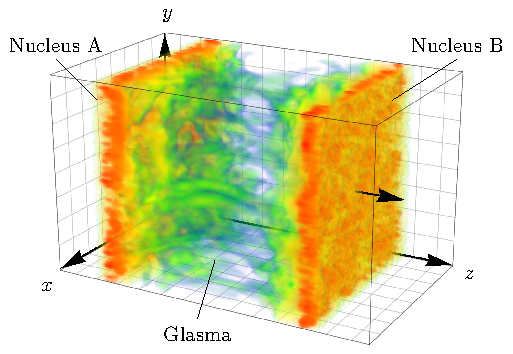
\includegraphics[height=0.8\paperheight]{images/fig1_overview.pdf}}};
}
\begin{frame}[plain,noframenumbering]{}
    \begin{center}
        \vspace{1cm}
        {\large\color{normal}Initial stage of pre-equilibrium}\\[0.3cm]
        {\huge\color{destacado}The glasma}
    \end{center}
\end{frame}
\setbeamertemplate{background}{}

%%%%%%%%%%%%%%%%%%%%%%%%%%%%%%%%%%%%%%%%%
%%%%%%%%%%%%%%%%% SLIDE %%%%%%%%%%%%%%%%%
%%%%%%%%%%%%%%%%%%%%%%%%%%%%%%%%%%%%%%%%%

\setbeamertemplate{background}{
\tikz[overlay,remember picture] \node[at=(current page.center), align=center] {\\[10pt]
{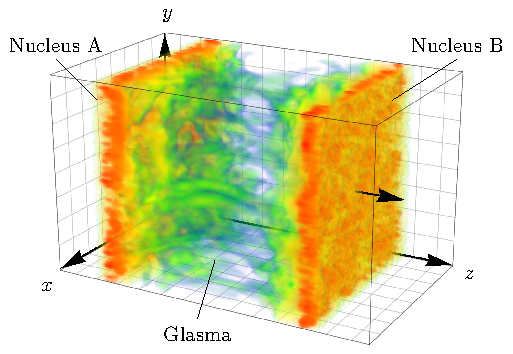
\includegraphics[height=0.7\paperheight]{images/fig1_overview.pdf}}};
}
\begin{frame}[plain,noframenumbering]
    \frametitle{\\ Glasma color fields}
    \blfootnote{\scriptsize Ipp, Müller  \href{https://arxiv.org/abs/1703.00017}{{\color{palgold}\texttt{[1703.00017]}$^\text{\tiny\faExternalLink}$}}}
\end{frame}
\setbeamertemplate{background}{}

%%%%%%%%%%%%%%%%%%%%%%%%%%%%%%%%%%%%%%%%%
%%%%%%%%%%%%%% SUBSECTION %%%%%%%%%%%%%%%
%%%%%%%%%%%%%%%%%%%%%%%%%%%%%%%%%%%%%%%%%

\subsection{CGC}

%%%%%%%%%%%%%%%%%%%%%%%%%%%%%%%%%%%%%%%%%
%%%%%%%%%%%%%%%%% SLIDE %%%%%%%%%%%%%%%%%
%%%%%%%%%%%%%%%%%%%%%%%%%%%%%%%%%%%%%%%%%

\begin{frame}
    \frametitle{CGC and glasma}
\end{frame}

%%%%%%%%%%%%%%%%%%%%%%%%%%%%%%%%%%%%%%%%%
%%%%%%%%%%%%%% SUBSECTION %%%%%%%%%%%%%%%
%%%%%%%%%%%%%%%%%%%%%%%%%%%%%%%%%%%%%%%%%

\subsection{Features}

%%%%%%%%%%%%%%%%%%%%%%%%%%%%%%%%%%%%%%%%%
%%%%%%%%%%%%%%%%% SLIDE %%%%%%%%%%%%%%%%%
%%%%%%%%%%%%%%%%%%%%%%%%%%%%%%%%%%%%%%%%%

\begin{frame}
    \frametitle{Features of glasma fields}
\end{frame}


%%%%%%%%%%%%%%%%%%%%%%%%%%%%%%%%%%%%%%%%%
%%%%%%%%%%%%%% SUBSECTION %%%%%%%%%%%%%%%
%%%%%%%%%%%%%%%%%%%%%%%%%%%%%%%%%%%%%%%%%

\subsection{Frameworks}

%%%%%%%%%%%%%%%%%%%%%%%%%%%%%%%%%%%%%%%%%
%%%%%%%%%%%%%%%%% SLIDE %%%%%%%%%%%%%%%%%
%%%%%%%%%%%%%%%%%%%%%%%%%%%%%%%%%%%%%%%%%

\begin{frame}
    \frametitle{Frameworks for glasma}
\end{frame}



%%%%%%%%%%%%%%%%%%%%%%%%%%%%%%%%%%%%%%%%%
%%%%%%%%%%%%%%%% SECTION %%%%%%%%%%%%%%%%
%%%%%%%%%%%%%%%%%%%%%%%%%%%%%%%%%%%%%%%%%

\section{Transport in glasma}

%%%%%%%%%%%%%%%%%%%%%%%%%%%%%%%%%%%%%%%%%
%%%%%%%%%%%%%% SUBSECTION %%%%%%%%%%%%%%%
%%%%%%%%%%%%%%%%%%%%%%%%%%%%%%%%%%%%%%%%%

\subsection{Classical transport}

%%%%%%%%%%%%%%%%%%%%%%%%%%%%%%%%%%%%%%%%%
%%%%%%%%%%%%%%%%% SLIDE %%%%%%%%%%%%%%%%%
%%%%%%%%%%%%%%%%%%%%%%%%%%%%%%%%%%%%%%%%%

\begin{frame}
    \frametitle{Wong's equations}
\end{frame}

%%%%%%%%%%%%%%%%%%%%%%%%%%%%%%%%%%%%%%%%%
%%%%%%%%%%%%%% SUBSECTION %%%%%%%%%%%%%%%
%%%%%%%%%%%%%%%%%%%%%%%%%%%%%%%%%%%%%%%%%

\subsection{Field correlators}

%%%%%%%%%%%%%%%%%%%%%%%%%%%%%%%%%%%%%%%%%
%%%%%%%%%%%%%%%%% SLIDE %%%%%%%%%%%%%%%%%
%%%%%%%%%%%%%%%%%%%%%%%%%%%%%%%%%%%%%%%%%

\begin{frame}
    \frametitle{Correlator method}
\end{frame}


%%%%%%%%%%%%%%%%%%%%%%%%%%%%%%%%%%%%%%%%%
%%%%%%%%%%%%%%%% SECTION %%%%%%%%%%%%%%%%
%%%%%%%%%%%%%%%%%%%%%%%%%%%%%%%%%%%%%%%%%

\section{Results}

% %%%%%%%%%%%%%%%%%%%%%%%%%%%%%%%%%%%%%%%%%
% %%%%%%%%%%%%%% SUBSECTION %%%%%%%%%%%%%%%
% %%%%%%%%%%%%%%%%%%%%%%%%%%%%%%%%%%%%%%%%%

% \subsection{Momentum broadening}

% %%%%%%%%%%%%%%%%%%%%%%%%%%%%%%%%%%%%%%%%%
% %%%%%%%%%%%%%%%%% SLIDE %%%%%%%%%%%%%%%%%
% %%%%%%%%%%%%%%%%%%%%%%%%%%%%%%%%%%%%%%%%%

% \begin{frame}
%     \frametitle{Momentum broadening}
% \end{frame}

%%%%%%%%%%%%%%%%%%%%%%%%%%%%%%%%%%%%%%%%%
%%%%%%%%%%%%%% SUBSECTION %%%%%%%%%%%%%%%
%%%%%%%%%%%%%%%%%%%%%%%%%%%%%%%%%%%%%%%%%

\subsection{Transport coefficients}

%%%%%%%%%%%%%%%%%%%%%%%%%%%%%%%%%%%%%%%%%
%%%%%%%%%%%%%%%%% SLIDE %%%%%%%%%%%%%%%%%
%%%%%%%%%%%%%%%%%%%%%%%%%%%%%%%%%%%%%%%%%

\begin{frame}
    \frametitle{Transport coefficients}
\end{frame}



%%%%%%%%%%%%%%%%%%%%%%%%%%%%%%%%%%%%%%%%%
%%%%%%%%%%%%%% SUBSECTION %%%%%%%%%%%%%%%
%%%%%%%%%%%%%%%%%%%%%%%%%%%%%%%%%%%%%%%%%

\subsection{Observables}

%%%%%%%%%%%%%%%%%%%%%%%%%%%%%%%%%%%%%%%%%
%%%%%%%%%%%%%%%%% SLIDE %%%%%%%%%%%%%%%%%
%%%%%%%%%%%%%%%%%%%%%%%%%%%%%%%%%%%%%%%%%

\begin{frame}
    \frametitle{Phenomenology}
\end{frame}

%%%%%%%%%%%%%%%%%%%%%%%%%%%%%%%%%%%%%%%%%
%%%%%%%%%%%%%%%% SECTION %%%%%%%%%%%%%%%%
%%%%%%%%%%%%%%%%%%%%%%%%%%%%%%%%%%%%%%%%%

\section{Open questions}

%%%%%%%%%%%%%%%%%%%%%%%%%%%%%%%%%%%%%%%%%
%%%%%%%%%%%%%% SUBSECTION %%%%%%%%%%%%%%%
%%%%%%%%%%%%%%%%%%%%%%%%%%%%%%%%%%%%%%%%%

%%%%%%%%%%%%%%%%%%%%%%%%%%%%%%%%%%%%%%%%%
%%%%%%%%%%%%%%%%% SLIDE %%%%%%%%%%%%%%%%%
%%%%%%%%%%%%%%%%%%%%%%%%%%%%%%%%%%%%%%%%%

\begin{frame}
    \frametitle{Open questions}
\end{frame}






\end{document}